\chapter{Experiments}
\label{c:experiments}
\IMRADlabel{results}



In this chapter we will present all environments we experimented with as well as \emph{hyper-experiments}, \ac{ie} experiments with the hyperparameters and their influence on the algorithm performance (in terms of the prediction error and similar metrics, not the computing time).

We split this chapter into two parts: Firstly, we will present the experiment setup we used and the different environments we tested on. Secondly, we present our results and put them in context of other results. All critical discussion and comparison with related work will take place in~\autoref{c:discussion}.

\section{Setup}
	In this section we will introduce the experiment setup and all the different environments we used for evaluation.

	\subsection{Environments}
		This section covers the different environments we used and changed we might have applied to them. Do generate the data, you have to run the file \texttt{src/data.py} with the desired experiment ID as the first argument, \ac{eg} \texttt{python src/data.py pendulum\_damped}. If no argument is given, a regeneration of the data from all experiments is triggered. For each of the following environments we summarize the most important data about the environment at the start of the subsection, including the experiment ID.

		\subsubsection{Proof-of-Concept: Classic LGDS}
			\begin{itemize}
				\item Experiment ID: \texttt{lgds}
			\end{itemize}

			As a proof-of-concept and to empirically verify our proof on the exactness of the cubature rule and hence the similar expected performance for plain linear systems, we benchmark our algorithm against a simple linear system. The linear system has a two-dimensional state \( \vec{y} \coloneqq \begin{bmatrix} x_1 & x_2 \end{bmatrix}^T \) with the dynamics
			\begin{align*}
				\dot{x}_1 &= x_2 \\
				\dot{x}_2 &= -x_1
			\end{align*}
			The initial state \( \vec{s}_1 \) is sampled from a Gaussian with mean \( \begin{bmatrix} 0.1 & 0.2 \end{bmatrix}^T \) and covariance \( \diag\big(10^{-5}, 10^{-5}\big) \). The system is integrated using the implicit Runge-Kutta Radau~IIA~\cite{guglielmiImplementingRadauIIA2001} method with an evaluation interval of \( h = 0.1 \) for \( T = 240 \) time steps where only the first \( T_\train = 120 \) steps are used for training and the remaining \(120\) are used for validation. The raw data is shown in~\autoref{fig:envLgds}.

			As the system's eigenvalues \( -i \), \( i \) are purely imaginary, the integrated system rings around the equilibrium \( \begin{bmatrix} 0 & 0 \end{bmatrix}^T \) infinitely.

			\begin{figure}
				\centering
				\begin{subfigure}{0.5\linewidth}
					\centering
					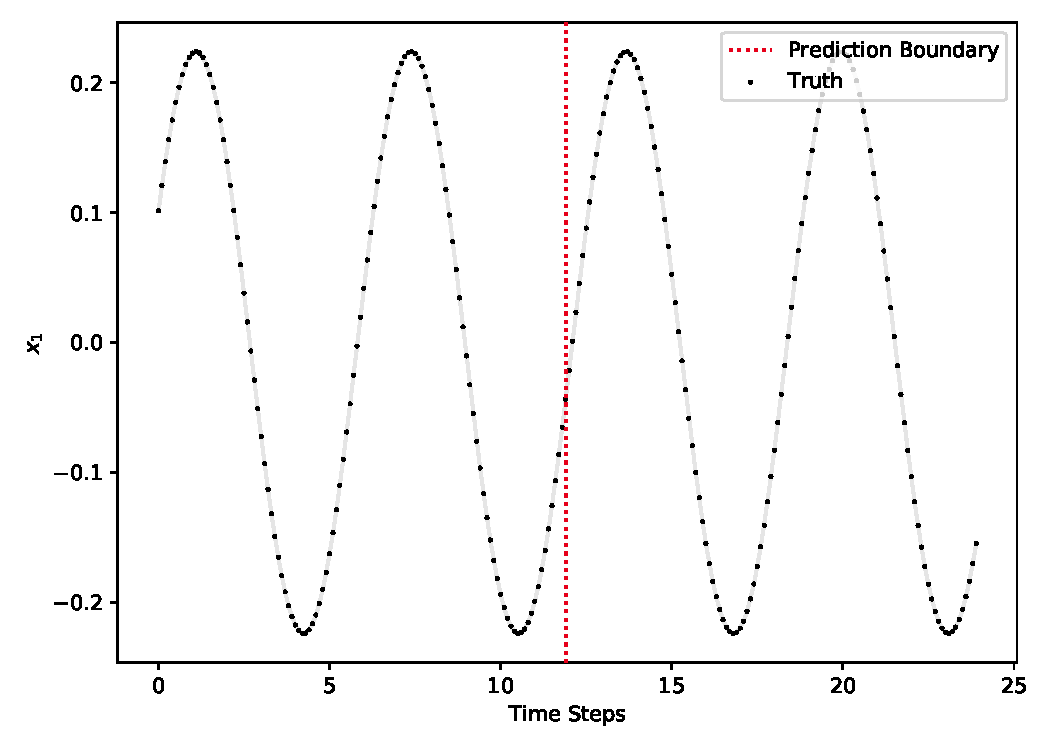
\includegraphics[width=\linewidth]{figures/experiments/environments/observations-lgds-N0-D0.pdf}
				\end{subfigure}%
				~
				\begin{subfigure}{0.5\linewidth}
					\centering
					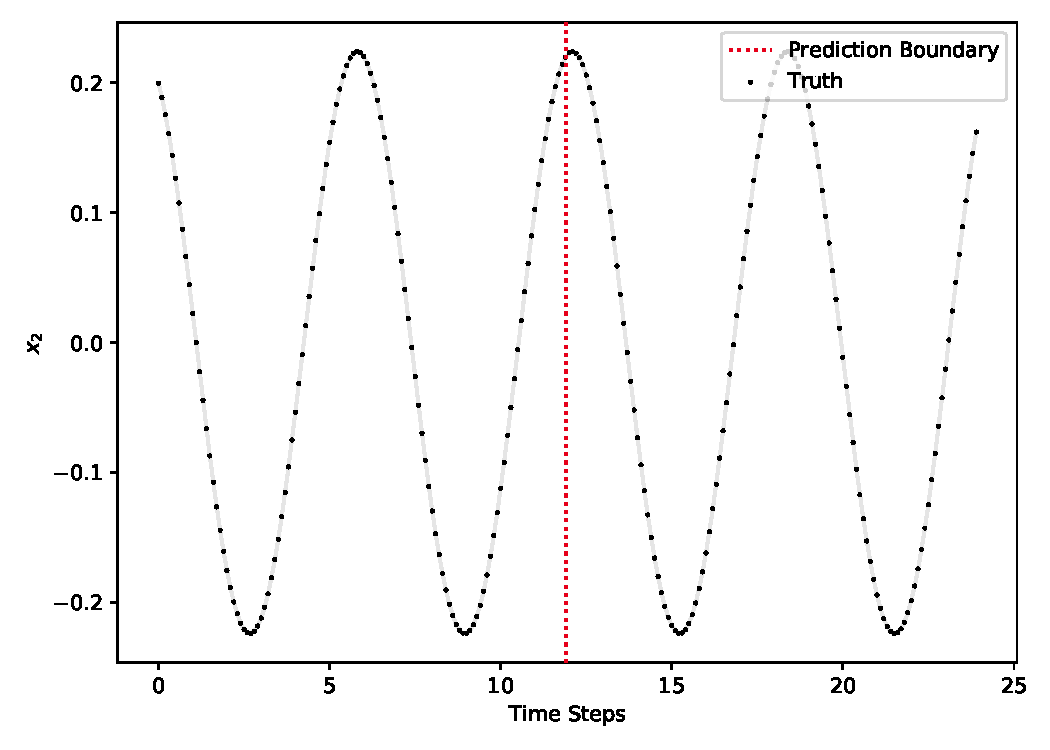
\includegraphics[width=\linewidth]{figures/experiments/environments/observations-lgds-N0-D1.pdf}
				\end{subfigure}
				\caption{Plot of the raw data used for training the proof-of-concept \ac{lgds} environment. The black dots represent the actual data points, all before the red prediction boundary are used for training, the rest for validation. The faint gray line emphasizes the connection between the data points and that they are actually generated from a dynamical system.}
				\label{fig:envLgds}
			\end{figure}
		% end

		\subsubsection{Proof-of-Concept: Polynomial}
			\begin{itemize}
				\item Experiment ID: \texttt{polynomial}
			\end{itemize}

			This is our second proof-of-concept and the first that actually proofs our concept of learning nonlinear dynamics with a linear embedding. For this environments we
		% end

		\subsubsection{(Damped) Pendulum}
			\begin{itemize}
				\item Experiment ID: \texttt{pendulum} and \texttt{pendulum\_damped}
			\end{itemize}

			The first nonlinear system we look at is the (inverted) pendulum in both an undamped and a damped setting. For this experiment, we use the angular state \( \vec{y} = \begin{bmatrix} \theta & \dot{\theta} \end{bmatrix} \) where \(\theta\) is the displacement angle (see~\autoref{fig:envPendulumSketch}). The dynamics are specified by the \ac{ode}
			\begin{equation*}
				\ddot{\theta} = \sin\theta - d \dot{\theta}
			\end{equation*}
			that is solved using the Radau~IIA~\cite{guglielmiImplementingRadauIIA2001} \ac{ivp} integrator (after transforming the \ac{ode} in a first-order \ac{ode} system). The initial velocity is set to \(0\) and the initial position is sampled from a Gaussian with mean \( \pi/36 \) and variance \( \pi/8 \). This puts the pendulum in motion as it falls down from its initial position. For the undamped pendulum, we set \( d = 0 \). For both environments, we use an evaluation interval of \( h = 0.1 \) for \( T = 1000 \) time steps where only the first \( T_\train = 500 \) steps are used for training and the remaining \(500\) are used for validation. The raw data is shown in~\autoref{fig:envPendulum} for the undamped and~\autoref{fig:envPendulumDamped} for the damped pendulum.

			The damped pendulum is especially interesting as the system looses energy (\ac{ie} the sum of the kinetic and potential energy decreases over time) and Koopman theory in general has problems with finding embeddings that are able to encode energy loss\todo{citation needed}.

			\begin{figure}
				\centering
				\begin{subfigure}{0.5\linewidth}
					\centering
					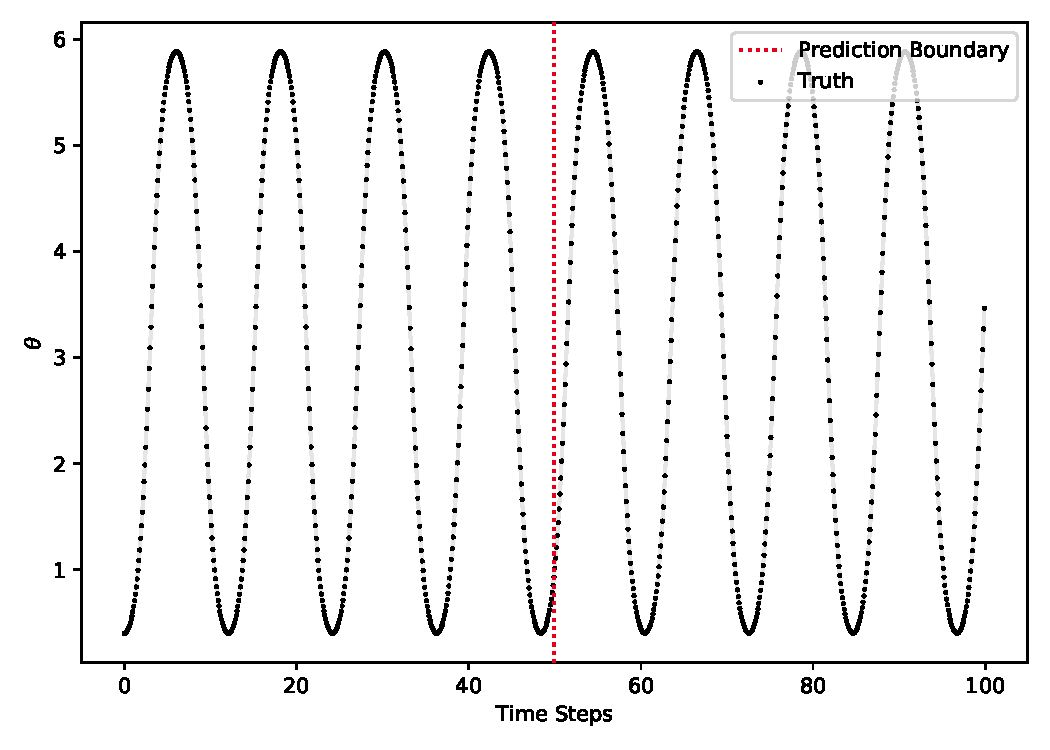
\includegraphics[width=\linewidth]{figures/experiments/environments/observations-pendulum-N0-D0.pdf}
				\end{subfigure}%
				~
				\begin{subfigure}{0.5\linewidth}
					\centering
					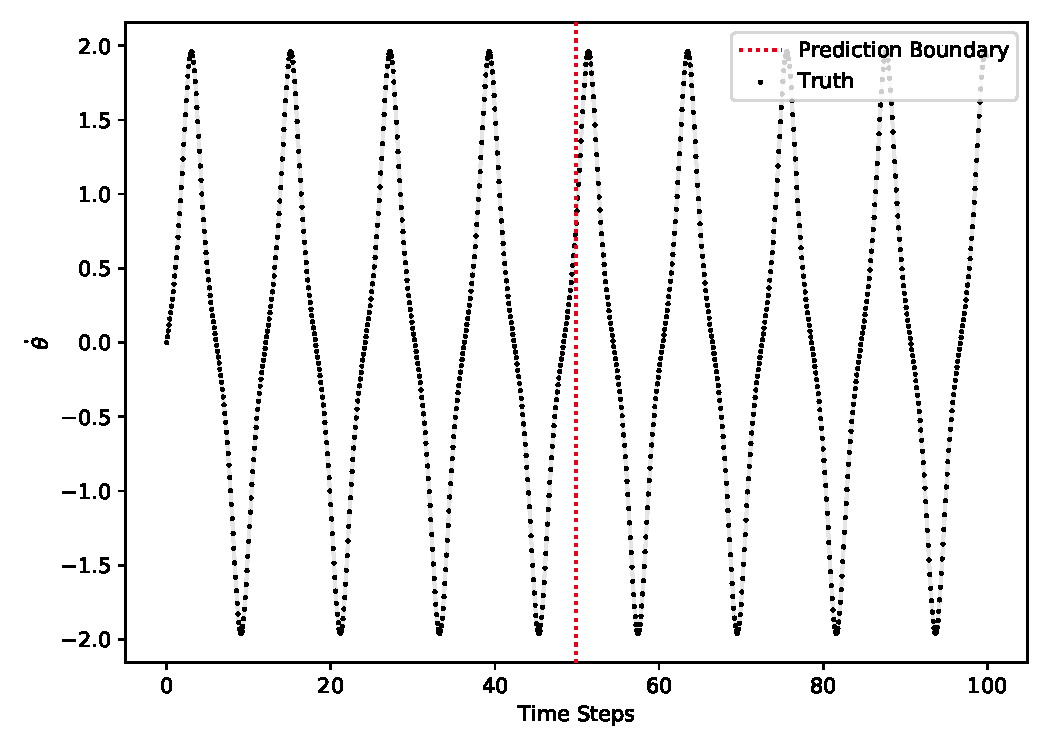
\includegraphics[width=\linewidth]{figures/experiments/environments/observations-pendulum-N0-D1.pdf}
				\end{subfigure}
				\caption{Plot of the raw data used for training the undamped pendulum environment. The black dots represent the actual data points, all before the red prediction boundary are used for training, the rest for validation. The faint gray line emphasizes the connection between the data points and that they are actually generated from a dynamical system.}
				\label{fig:envPendulum}
			\end{figure}
			\begin{figure}
				\centering
				\begin{subfigure}{0.5\linewidth}
					\centering
					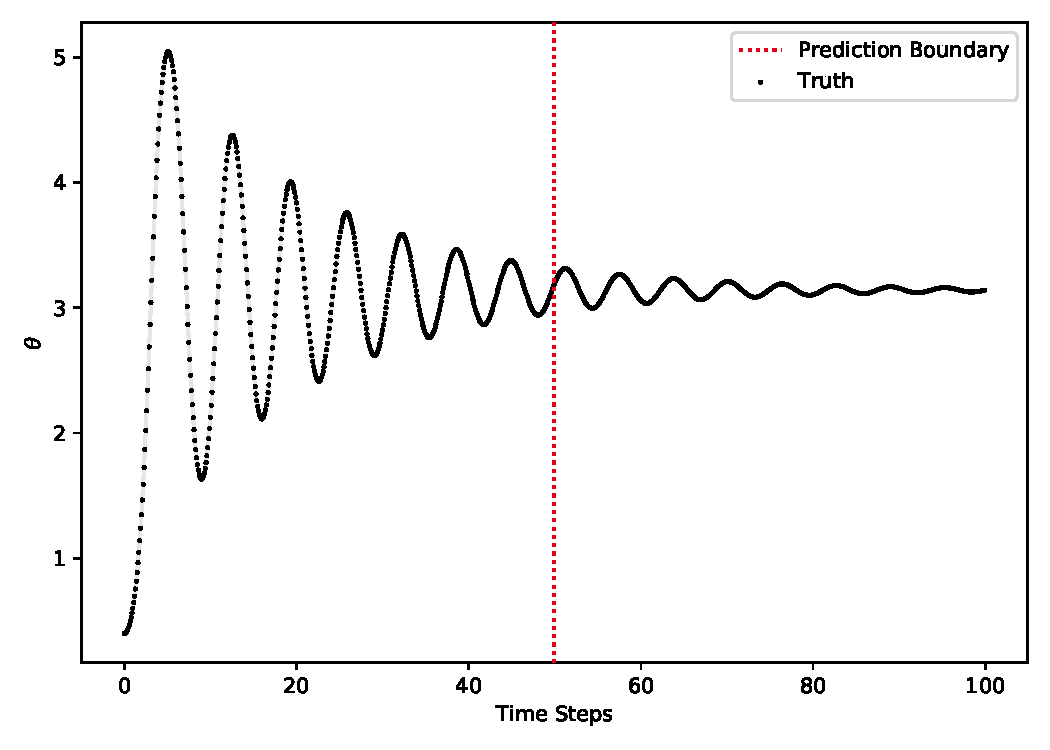
\includegraphics[width=\linewidth]{figures/experiments/environments/observations-pendulum-damped-N0-D0.pdf}
				\end{subfigure}%
				~
				\begin{subfigure}{0.5\linewidth}
					\centering
					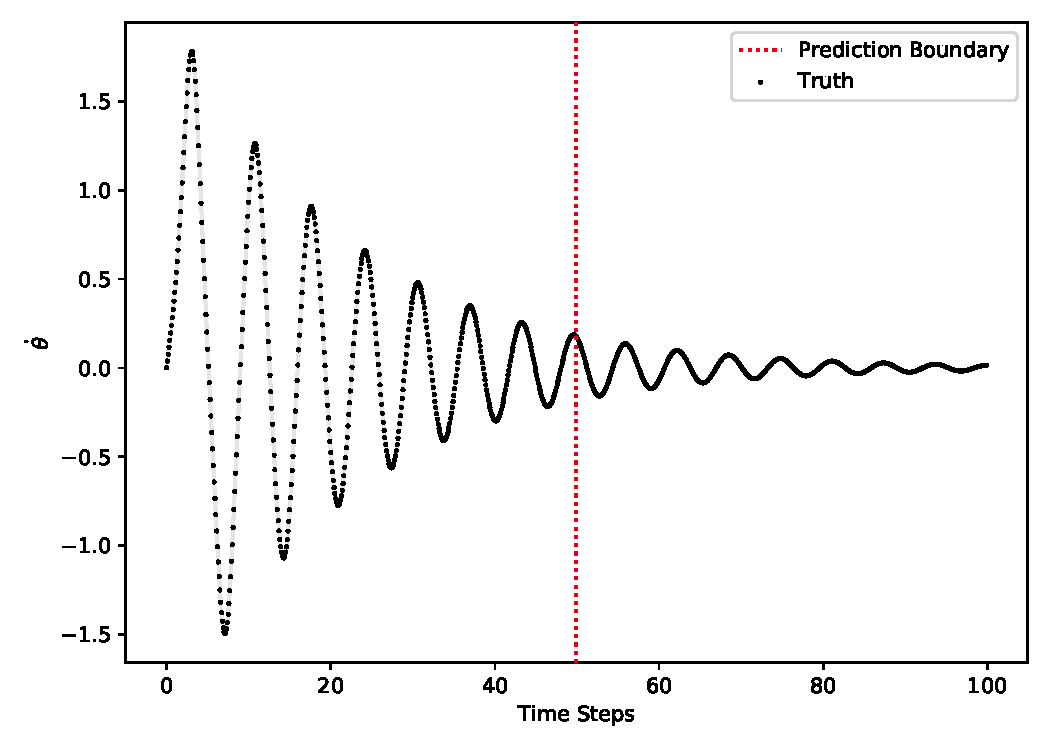
\includegraphics[width=\linewidth]{figures/experiments/environments/observations-pendulum-damped-N0-D1.pdf}
				\end{subfigure}
				\caption{Plot of the raw data used for training the damped pendulum environment. The black dots represent the actual data points, all before the red prediction boundary are used for training, the rest for validation. The faint gray line emphasizes the connection between the data points and that they are actually generated from a dynamical system.}
				\label{fig:envPendulumDamped}
			\end{figure}

			\begin{figure}
				\centering
				\tikzSimplePendulum
				\caption{Illustration of the pendulum environment. The pendulum has length \(L\) and mass \(m\) and is attached to a fixed point in the center around which it can swing. In the case of the undamped pendulum, it swings freely, otherwise it is damped with a damping constant \(d\).}
				\label{fig:envPendulumSketch}
			\end{figure}
		% end

		\subsubsection{Gym Pendulum}
			\begin{itemize}
				\item Experiment ID: \texttt{pendulum\_gym}
			\end{itemize}

			This is a sine/cosine version of the pendulum introduced before, but without damping. We use the environment of OpenAI Gym~\cite{brockmanOpenAIGym2016} for generating the data used for training. The motion equations are still the same as for the non-Gym pendulum
			\begin{equation*}
				\ddot{\theta} = \sin\theta
			\end{equation*}
			with \( d = 0 \) as the Gym pendulum does not include damping, but the state is defined as the sine and cosine of the angle:
			\begin{equation*}
				\vec{y} \coloneqq
					\begin{bmatrix}
						\cos\theta \\
						\sin\theta \\
						\dot{\theta}
					\end{bmatrix}
			\end{equation*}
			The Gym environment uses the Euler method for integrating the \ac{ode} with a step size of \( h = 0.05 \). We generate \( T = 100 \) time steps of which \( T_\train = 50 \) are used for training and the other \(50\) for validation. The raw data is shown in~\autoref{fig:envPendulumGym}.

			\begin{figure}
				\centering
				\begin{subfigure}{0.5\linewidth}
					\centering
					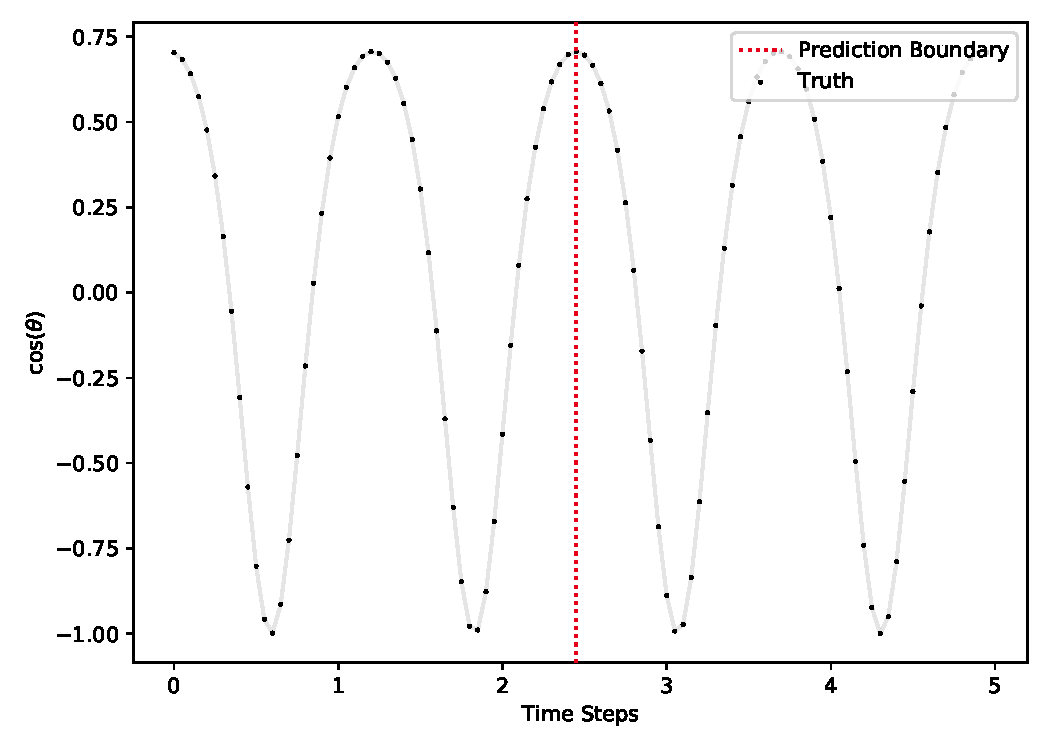
\includegraphics[width=\linewidth]{figures/experiments/environments/observations-pendulum-gym-N0-D0.pdf}
				\end{subfigure}%
				~
				\begin{subfigure}{0.5\linewidth}
					\centering
					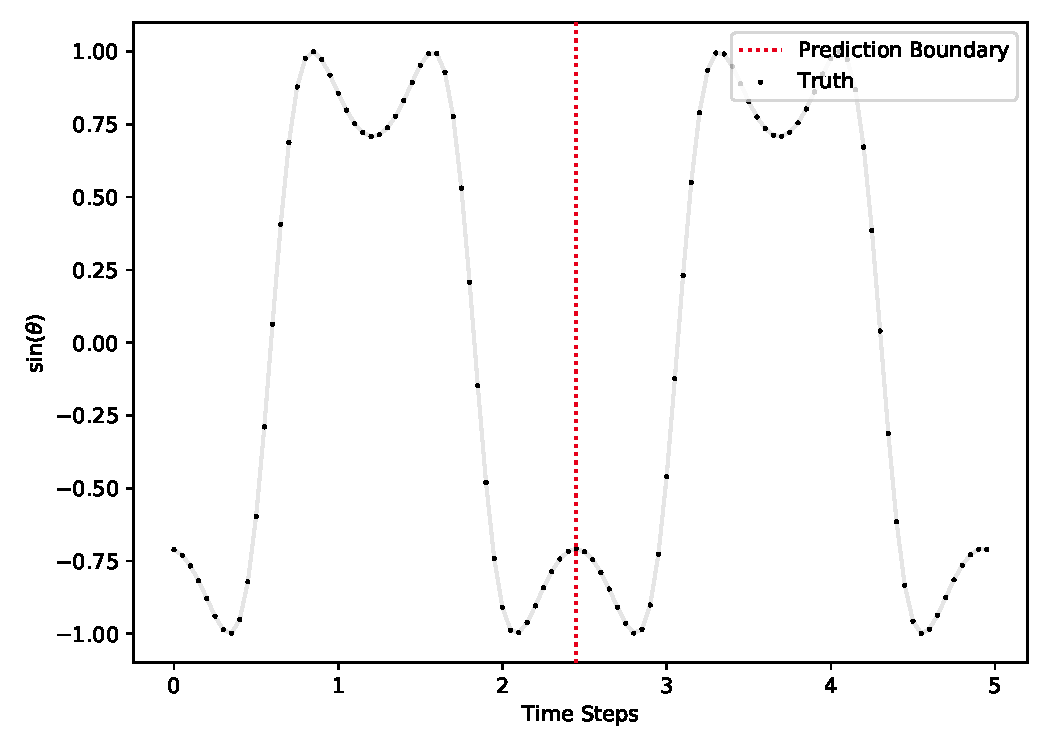
\includegraphics[width=\linewidth]{figures/experiments/environments/observations-pendulum-gym-N0-D1.pdf}
				\end{subfigure} \\
				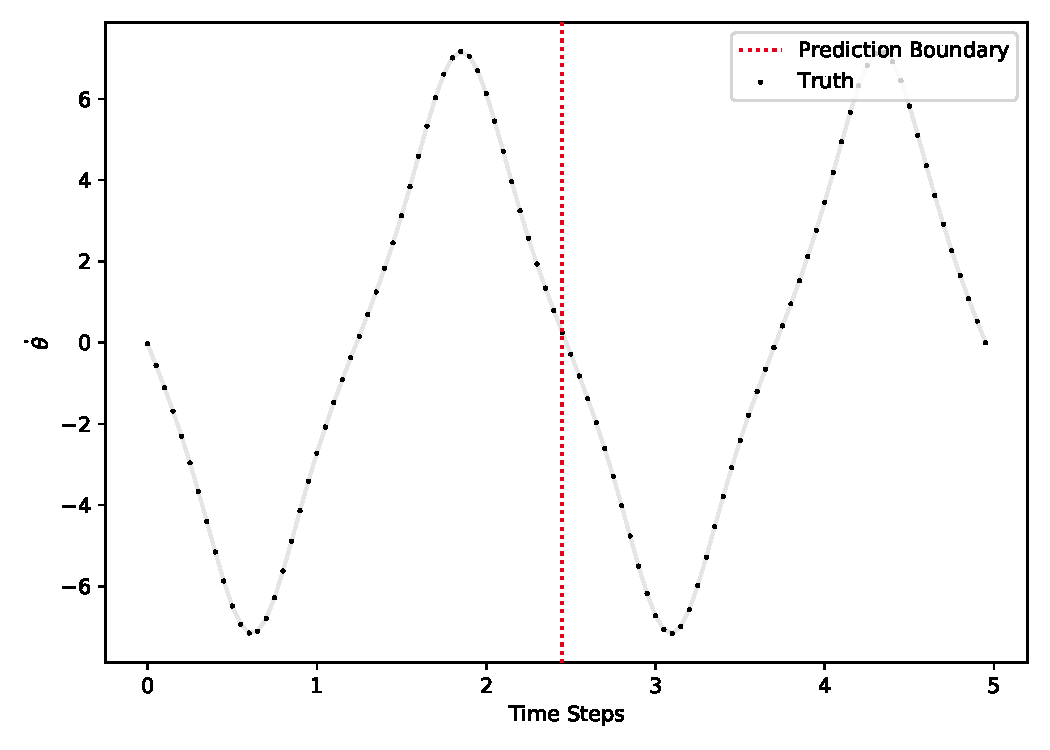
\includegraphics[width=0.5\linewidth]{figures/experiments/environments/observations-pendulum-gym-N0-D2.pdf}
				\caption{Plot of the raw data used for training the Gym pendulum environment. The black dots represent the actual data points, all before the red prediction boundary are used for training, the rest for validation. The faint gray line emphasizes the connection between the data points and that they are actually generated from a dynamical system.}
				\label{fig:envPendulumGym}
			\end{figure}
		% end

		\subsubsection{Gym Cartpole}
			\label{subsubsec:cartpole}

			\begin{itemize}
				\item Experiment ID: \texttt{cartpole\_gym}
			\end{itemize}

			The second last environment we run experiment on is the cartpole environment. In the cartpole environment, an inverted pendulum is build on a (typically controlled, but otherwise freely movable) cart. If the pendulum falls town, the torque on the joint is translated into a force moving the cart around. This creates nonlinear coupling and therefore highly nonlinear dynamics. A sketch of the cartpole environment is given in~\autoref{fig:envCartpoleGymSketch}. As for the previous pendulum, we rely on the cartpole implementation of Gym. We slightly modified the environment to be uncontrolled, as the environment usually has discrete actions for pushing the cart left or right. This modification is shown in~\autoref{lst:uncontrolledCartPole}. The state of the environment is given as
			\begin{equation*}
				\vec{y} \coloneqq
					\begin{bmatrix}
						x \\
						\dot{x} \\
						\theta \\
						\dot{\theta}
					\end{bmatrix}
			\end{equation*}
			where \(x\) is the cart position, \(\dot{x}\) is the cart velocity, \(\theta\) is the pole angle and \(\dot{\theta}\) is the angular velocity. The implemented equations of movement, taken from~\cite{florianCorrectEquationsDynamics2005}, are given as
			\begin{align*}
				\ddot{\theta} &= \frac{g \sin\theta + \cos\theta \Big(\! \frac{-F - m_p \ell \dot{\theta}^2 \sin\theta}{m_c + m_p} \!\Big)}{\ell \Big(\! \frac{4}{3} - \frac{m_p \cos^2\theta}{m_c + m_p} \!\Big)} \\
				\ddot{x} &= \frac{F + m_p \ell \big( \dot{\theta}^2 \sin\theta - \ddot{\theta} \cos\theta \big)}{m_c + m_p}
			\end{align*}
			where \( g = \SI{9.81}{\meter\per\second\squared} \) is the gravitational acceleration, \( m_p = \SI{0.1}{\kilogram} \) and \( m_c = \SI{1}{\kilogram} \) are the masses of the pole and cart, respectively, \( 2\ell = \SI{1}{\meter} \) is the pole length and \( [F] = \si{\newton} \) is the external (control) force acting on the cart that we set to \( \SI{0}{\newton} \). The Gym environment uses the Euler method for integrating the \ac{ode} with a step size of \( h = 0.02 \). We generate \( T = 300 \) time steps of which we use \( T_\train = 150 \) for training and the remaining \(150\) steps for validation. The raw data is shown in~\autoref{fig:envCartpoleGym}.

			\begin{lstlisting}[caption={Modification of Gym's cartpole environment to get an uncontrolled cartpole.}, label=lst:uncontrolledCartPole]
from gym.envs.classic_control import CartPoleEnv

class UncontrolledCartPole(CartPoleEnv):
	def __init__(self):
	super().__init__()

	self.force_mag = 0.0
			\end{lstlisting}

			\begin{figure}
				\centering
				\tikzCartpole
				\caption{Illustration of the cartpole environment. The cart has mass \(m_c\), the pole \(m_p\) with length \(L\). The cart can move freely on the \(x\) axis, while the pendulum can swing freely around the center of the cart, causing it to move.}
				\label{fig:envCartpoleGymSketch}
			\end{figure}

			\begin{figure}
				\centering
				\begin{subfigure}{0.5\linewidth}
					\centering
					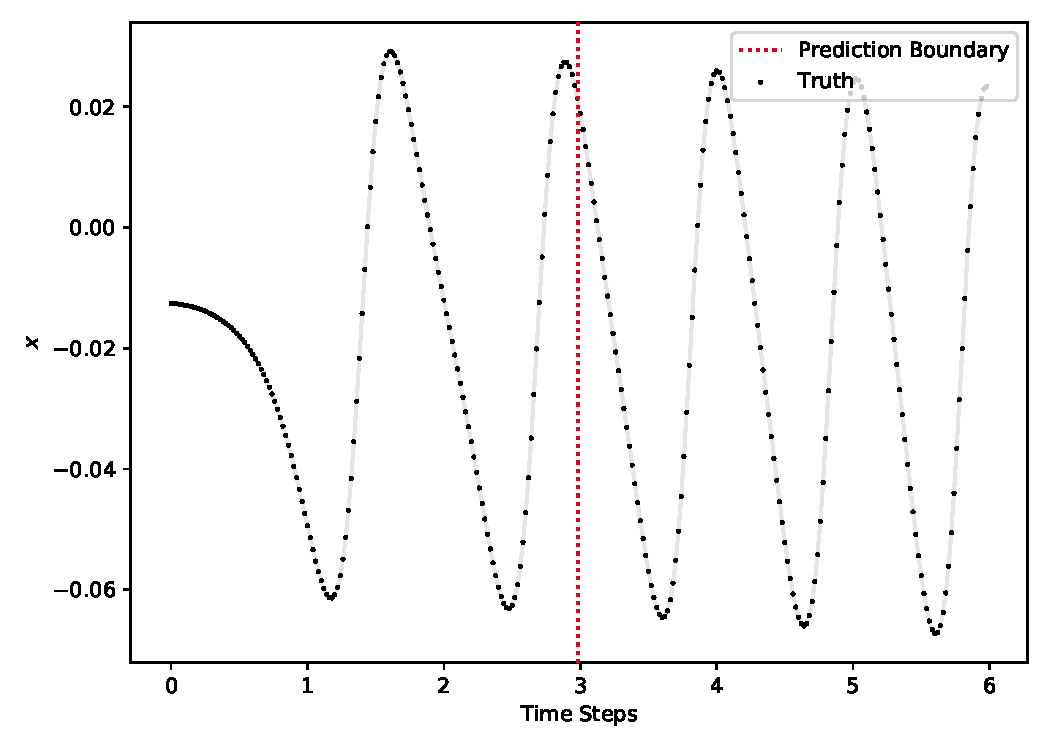
\includegraphics[width=\linewidth]{figures/experiments/environments/observations-cartpole-gym-N0-D0.pdf}
				\end{subfigure}%
				~
				\begin{subfigure}{0.5\linewidth}
					\centering
					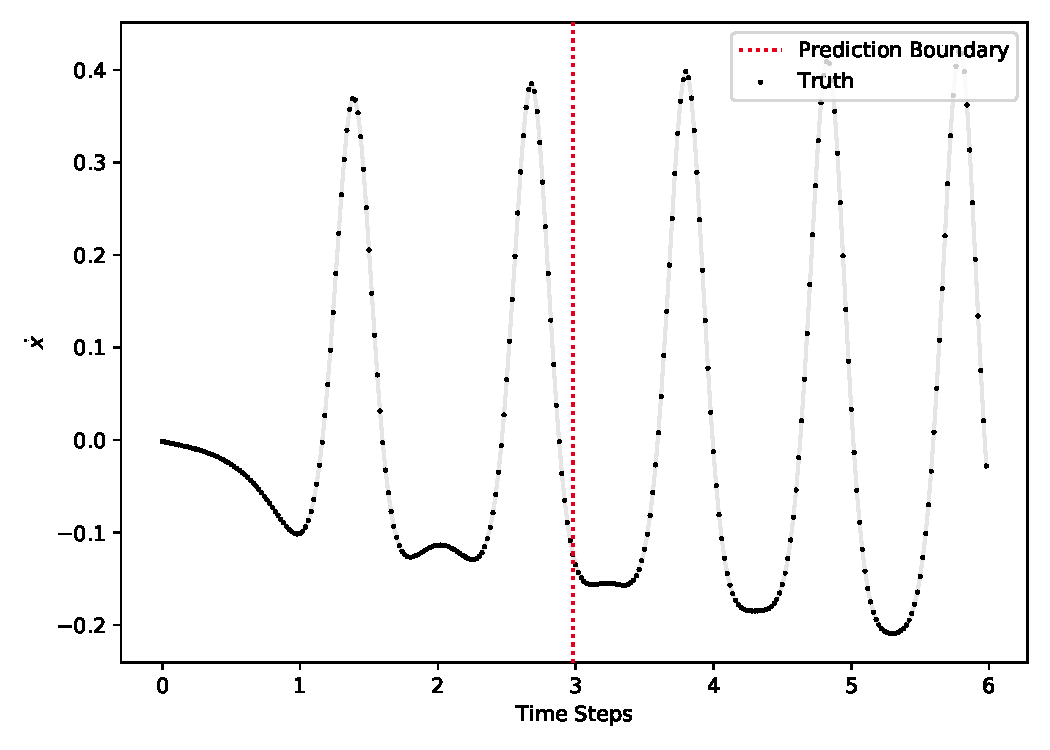
\includegraphics[width=\linewidth]{figures/experiments/environments/observations-cartpole-gym-N0-D1.pdf}
				\end{subfigure} \\
				\begin{subfigure}{0.5\linewidth}
					\centering
					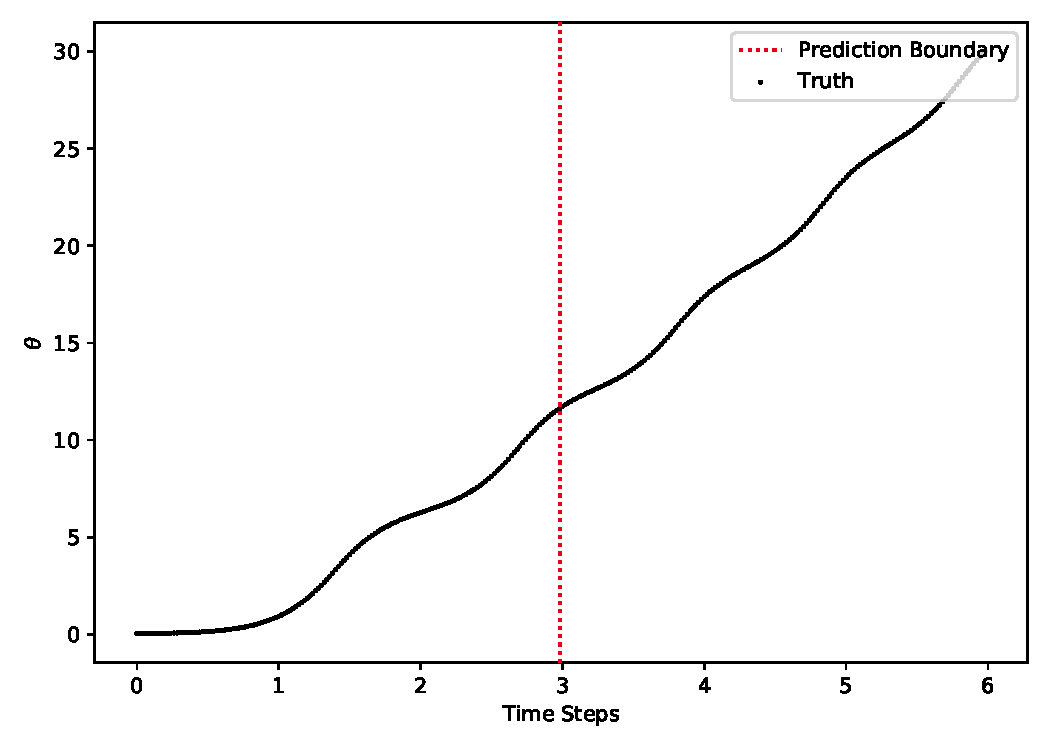
\includegraphics[width=\linewidth]{figures/experiments/environments/observations-cartpole-gym-N0-D2.pdf}
				\end{subfigure}%
				~
				\begin{subfigure}{0.5\linewidth}
					\centering
					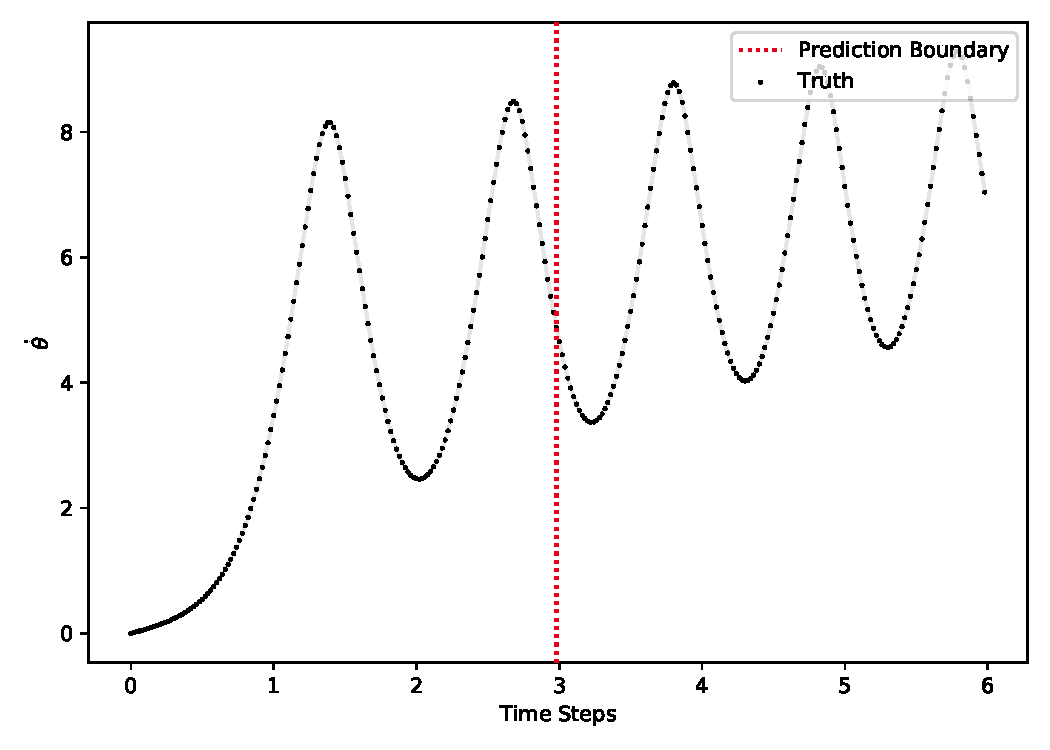
\includegraphics[width=\linewidth]{figures/experiments/environments/observations-cartpole-gym-N0-D3.pdf}
				\end{subfigure}
				\caption{Plot of the raw data used for training the Gym cartpole environment. The black dots represent the actual data points, all before the red prediction boundary are used for training, the rest for validation. The faint gray line emphasizes the connection between the data points and that they are actually generated from a dynamical system.}
				\label{fig:envCartpoleGym}
			\end{figure}
		% end

		\subsubsection{Gym Double Pendulum}
			\begin{itemize}
				\item Experiment ID: \texttt{acrobot\_gym}
			\end{itemize}

			The last environment we test is the double pendulum, implemented in Gym as the \emph{acrobot} (as for the cartpole, we removed all control inputs and modified the initial state to start on top rather than hanging straight down, see~\autoref{lst:topAcrobot}). The double pendulum consists of a pendulum on a fixed joint and a second pendulum attached to the end of the first pendulum. This creates highly nonlinear coupling and is the most common example of a chaotic system~\cite{shinbrotChaosDoublePendulum1992}. We observe the state vector
			\begin{equation*}
				\vec{y} \coloneqq
					\begin{bmatrix}
						\cos\varphi_1 \\
						\sin\varphi_1 \\
						\cos\varphi_2 \\
						\sin\varphi_2 \\
						\dot{\varphi}_1 \\
						\dot{\varphi}_2
					\end{bmatrix}
			\end{equation*}
			where \(\varphi_1\) and \(\varphi_2\) are the displacement of the first and second joint, respectively. See~\autoref{fig:envDoublePendulumGymSketch}) for a sketch of the double pendulum. The governing equations of motion are given as:´
			\begin{align*}
				\ddot{\varphi}_1 &= \frac{g (\sin\varphi_2 \, \cos\varphi_\Delta - \mu \sin\varphi_1) - (\ell_2 \dot{\varphi}_2^2 + \ell_1 \dot{\varphi}_1^2 \cos\varphi_\Delta) \sin\varphi_\Delta}{\ell_1 (\mu - \cos^2\varphi_\Delta)} \\
				\ddot{\varphi}_2 &= \frac{g \mu (\sin\varphi_2 \, \cos\varphi_\Delta - \mu \sin\varphi_1) + (\mu \ell_1 \dot{\varphi}_1^2 + \ell_2 \dot{\varphi}_2^2 \cos\varphi_\Delta) \sin\varphi_\Delta}{\ell_2 (\mu - \cos^2\varphi_\Delta)}
			\end{align*}
			with \( \varphi_\Delta \coloneqq \varphi_1 - \varphi \), \( \mu \coloneqq 1 + m_1/m_2 \) where \( g = \SI{9.8}{\meter\per\second\squared} \) is the gravitational acceleration, \( m_1 = \SI{1}{\kilogram} \) and \( m_2 = \SI{1}{\kilogram} \) are the masses of the two links and \( \ell_1 = \SI{1}{\meter} \) and \( \ell_2 = \SI{1}{\meter} \) are the lengths of the two links. The Gym environment uses a \ac{rk4} for integrating the \ac{ode} with an evaluation interval of \( h = 0.2 \). We modified the initial position to be drawn from a Gaussian with mean \( \pi \) and standard deviation \( \pi/8 \) and the initial velocity to be drawn from a uniform distribution in the interval \( [-0.1, 0.1] \). We generate \( T = 100 \) time steps of which we use \( T_\train = 75 \) for training and the remaining \(25\) for validation. The raw data is shown in~\autoref{fig:envDoublePendulumGym}.

			\begin{lstlisting}[caption={Modification of Gym's acrobot environment to start at the top instead of hanging down.}, label=lst:topAcrobot]
import numpy as np
from gym.envs.classic_control import AcrobotEnv

class ModifiedAcrobotEnv(AcrobotEnv):
	def __init__(self):
		super().__init__()

	def reset(self):
		position = self.np_random.normal(np.pi, np.pi / 8.0, size=(2,))
		velocity = self.np_random.uniform(low=-0.1, high=0.1, size=(2,))
		self.state = np.concatenate([position, velocity], axis=0)
		return self._get_ob()
			\end{lstlisting}

			\begin{figure}
				\centering
				\tikzDoublePendulum
				\caption{Illustration of the double pendulum environment. The pendulums have lengths \(\ell_1\) and \(\ell_2\) with the masses \(m_1\) and \(m_2\) attached to the respective ends. The inner pendulum can swing freely around the center while the other pendulum can swing freely around the end of the inner pendulum. Hence fixing one of the pendulums would transform the system back to a simple pendulum. If both pendulums can swing, the system is chaotic.}
				\label{fig:envDoublePendulumGymSketch}
			\end{figure}

			\begin{figure}
				\centering
				\begin{subfigure}{0.5\linewidth}
					\centering
					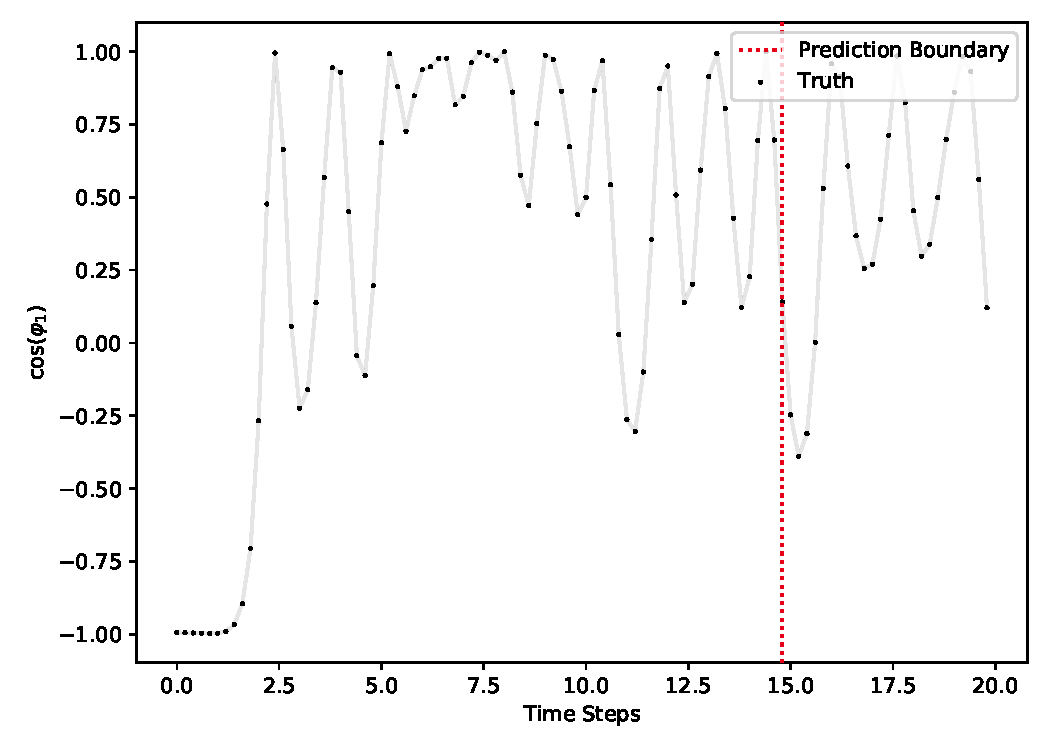
\includegraphics[width=\linewidth]{figures/experiments/environments/observations-acrobot-gym-N0-D0.pdf}
				\end{subfigure}%
				~
				\begin{subfigure}{0.5\linewidth}
					\centering
					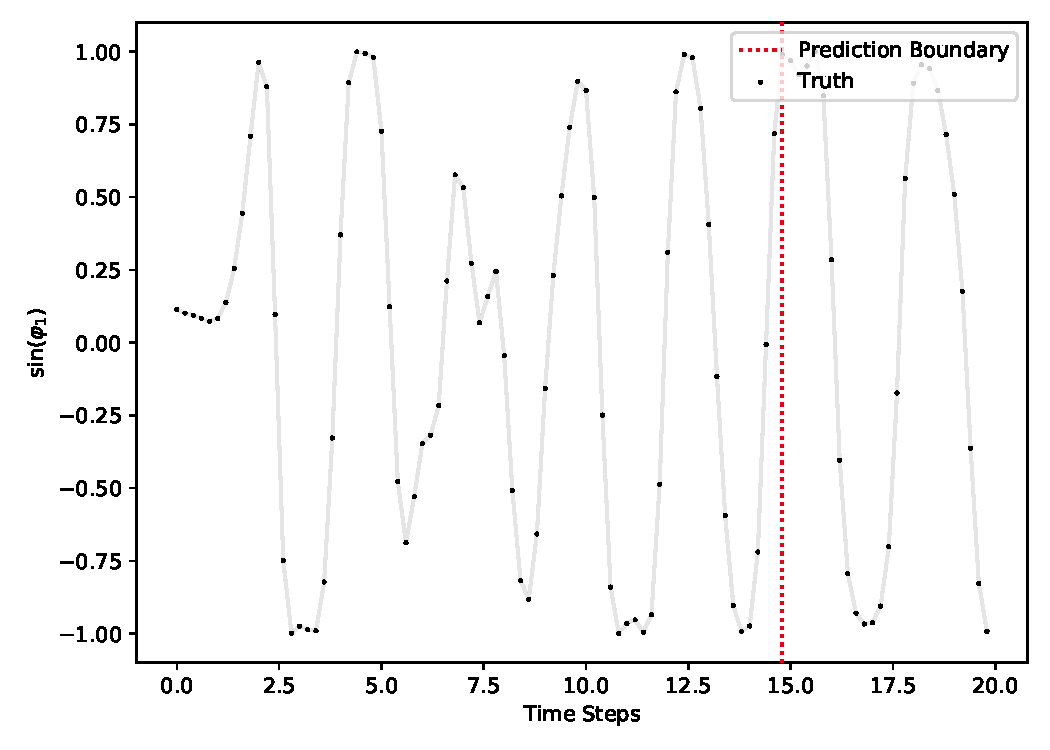
\includegraphics[width=\linewidth]{figures/experiments/environments/observations-acrobot-gym-N0-D1.pdf}
				\end{subfigure} \\
				\begin{subfigure}{0.5\linewidth}
					\centering
					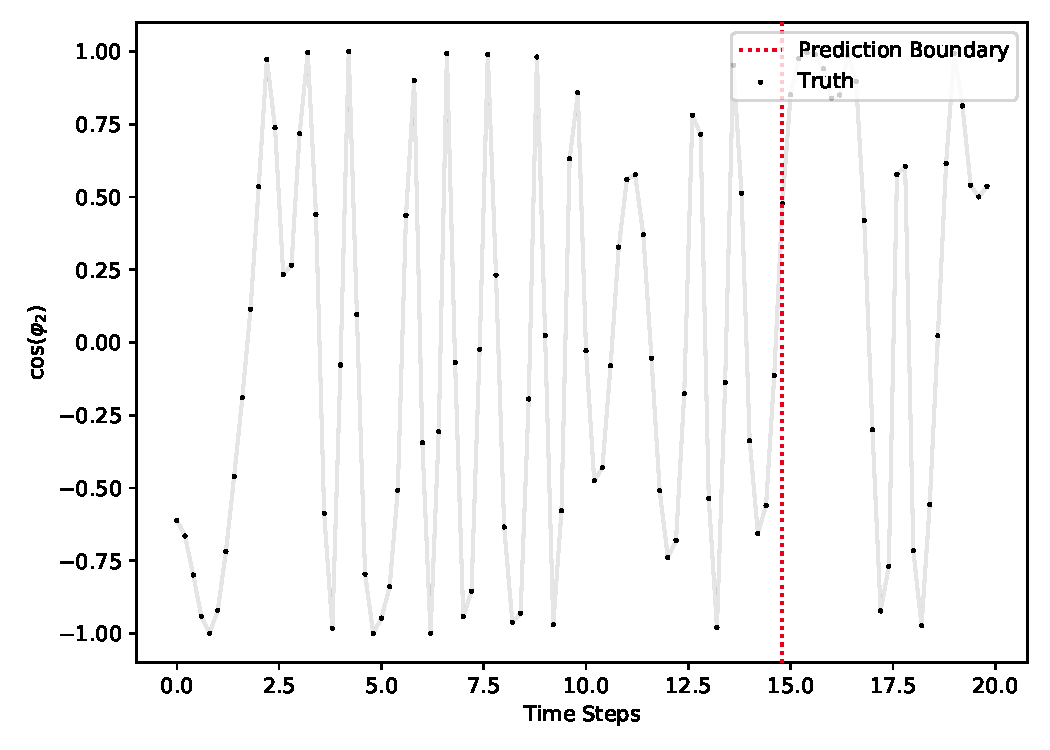
\includegraphics[width=\linewidth]{figures/experiments/environments/observations-acrobot-gym-N0-D2.pdf}
				\end{subfigure}%
				~
				\begin{subfigure}{0.5\linewidth}
					\centering
					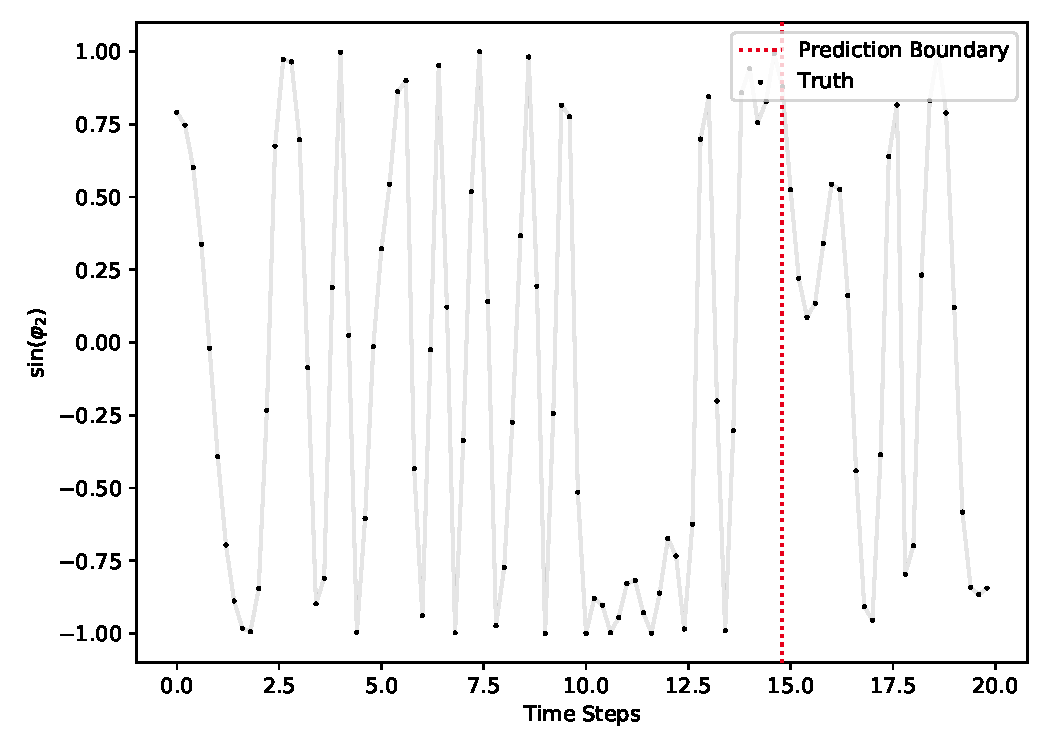
\includegraphics[width=\linewidth]{figures/experiments/environments/observations-acrobot-gym-N0-D3.pdf}
				\end{subfigure} \\
				\begin{subfigure}{0.5\linewidth}
					\centering
					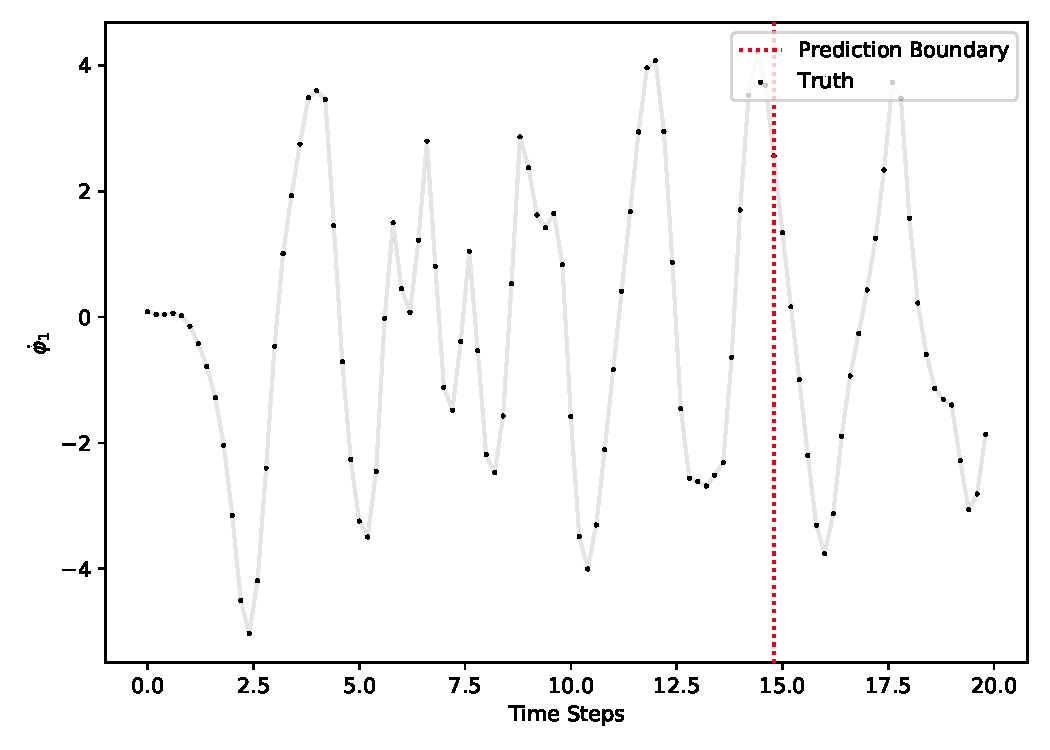
\includegraphics[width=\linewidth]{figures/experiments/environments/observations-acrobot-gym-N0-D4.pdf}
				\end{subfigure}%
				~
				\begin{subfigure}{0.5\linewidth}
					\centering
					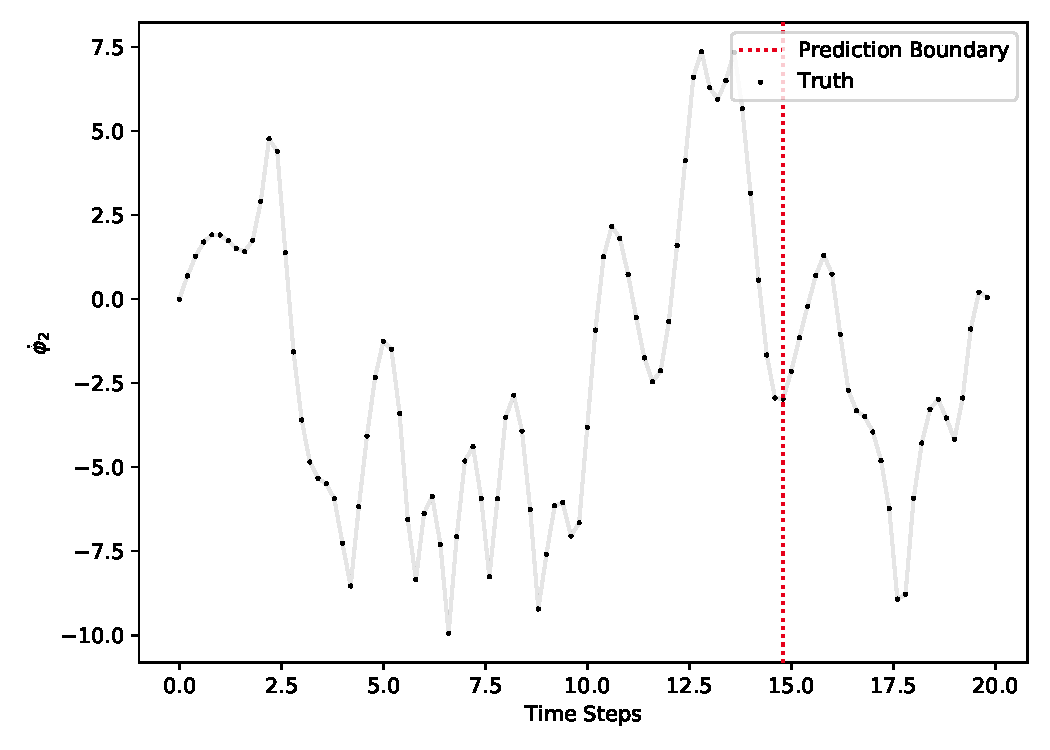
\includegraphics[width=\linewidth]{figures/experiments/environments/observations-acrobot-gym-N0-D5.pdf}
				\end{subfigure}
				\caption{Plot of the raw data used for training the Gym double pendulum environment. The black dots represent the actual data points, all before the red prediction boundary are used for training, the rest for validation. The faint gray line emphasizes the connection between the data points and that they are actually generated from a dynamical system.}
				\label{fig:envDoublePendulumGym}
			\end{figure}
		% end
	% end

	\subsection{Experiment Setup}
		We will now introduce the experiment setup, initialization and similar stuff we used for each environment. For all experiments, we initialized the latent state dynamics matrix \( \mat{A} \) with an identity matrix, the initial state \( \vec{m}_0 \) with a one-vector and all covariance matrices \( \mat{R} \), \( \mat{R} \) and \( \mat{V}_0 \) with a small diagonal covariance of \( 10^{-5} \). We set the maximum number of \(\vec{g}\)-optimization iterations to \(1000\) for all environments. As described in~\autoref{sec:implementation}, we used a neural network for the observation function with \(\tanh\) activation functions (except for the output layer of course) and a single hidden layer with \(50\) neurons. The environment-specific parameters and the hidden layer sizes are given in~\autoref{tab:experimentSetup}.

		\todo{Update table once more results are here and we changed hyperparameters!}
		\begin{table}
			\centering
			\begin{tabular}{c|ccc}
				\textbf{Environment} & \textbf{Whitening?} & \textbf{Latent Dim.} & \textbf{Max. Iterations} \\ \hline
				      Pendulum       &         no          &        \(10\)        &         \(100\)          \\
				  Damped Pendulum    &         yes         &        \(10\)        &         \(200\)          \\
				    Gym Pendulum     &         no          &        \(10\)        &         \(500\)          \\
				    Gym Cartpole     &         yes         &        \(8\)         &         \(500\)          \\
				    Gym Acrobot      &         no          &        \(16\)        &         \(350\)
			\end{tabular}
			\caption{Overview over the different hyperparameter setting for the different environments.}
			\label{tab:experimentSetup}
		\end{table}

		For the proof-of-concept environments (the linear system and the polynomial system), we used slightly different setups as those environments are a lot simpler. For the linear system, we used a zero-layer neural network with no activation function, \ac{ie} a learnable matrix/linear transformation. We also fix the latent dimensionality to be \(2\) for the linear system as we only have two states. For the polynomial system, we know~\cite{williamsonLearningNonLinearDynamical2020} that the Koopman operator has the exact finite form
		\begin{equation*}
			\mat{K} =
				\begin{bmatrix}
					\mu & 0       & 0        \\
					0   & \lambda & -\lambda \\
					0   & 0       & 2\mu
				\end{bmatrix}
		\end{equation*}
		with the Koopman observations \( \big(x_1, x_2, x_1^2\big) \). However, as we seek the \emph{inverse} Koopman observations, we chose a single hidden layer neural network with \(10\) hidden neurons and \(\tanh\) activation function and \(10000\) maximum \(\vec{g}\)-optimization iterations.
	% end

	\subsection{Hyper-Experiments}
		Besides the performance on specific environments, we where interested in how hyperparameters like the latent dimensionality affect the performance of the system. In this section we will discuss and present our experiment setup for the "hyper-experiments". All hyperparameters that are not part of the experiment where set to the ones listed in~\autoref{tab:experimentSetup}.

		If not stated differently, we always ran the experiment with five different seeds\footnote{Namely, we used the seeds \(0\), \(11\), \(42\), \(1234\) and \(1997\) that where chosen on a random basis.} to average out initialization noise.

		\subsubsection{Influence of the Latent Dimensionality}
			\label{subsec:experimentLatentDim}

			As the latent dimensionality directly influences how well the Koopman matrix can approximate the infinite-dimensional operator, it is one of the most interesting hyperparameters we evaluated. Hence, we evaluated lots of different latent dimensionalities from \( k = 1 \) to \( k = 50 \) (for cartpole, we did \( k = 1, 2, \rangedots, 100 \)).
		% end
	% end
% end

\section{Results}
	In this section we will look at the results of the experiments described above. We organized the section into the different environments and will take a look at both the hyper-experiments first and then the individual results for optimized hyperparameters.

	For evaluating the performance of the model, we use different measures and metrics, both qualitative and quantitative. For a qualitative evaluation, we simply plot the produced data. These plots can get quite noisy as we will see, but they comprise all things we need for a qualitative assessment:
	\begin{itemize}
		\item The \emph{ground truth}, generated as described above with the adequate numerical integration of the equations of motion.
		\item The \emph{smoothed states} as they are produced from the E-step of the \algname algorithm, \ac{ie} \(\hat{\vec{s}}_{1:T}\).
		\item The \emph{rollout}, starting both from the learned initial value as well as from the last smoothed state. While the former visualizes the ability of the model to work completely "on its own", the latter shows how well the linear dynamics generalize beyond the training data.
		\item And of course the confidence (\ac{ie} the learned variance) around each trajectory.
	\end{itemize}
	For quantitative comparison, we focus on the \ac{rmse} across all dimensions and time steps, where we can compute four different error values: The error over the rollout from start to finish (\( t = 1, 2, \rangedots, T \)), over the training data only (\( t = 1, 2, \rangedots, T_\train \)), over the prediction only (\( t = T_\train, T_\train + 1, \rangedots, T \)) or over the smoothed trajectory (\ac{ie} the results from the E-step, \(  \hat{\vec{s}}_{1:T} \)). The latter primarily checks that our algorithm performs correct and that it is even capable of learning the dynamics and it should be near zero or at least below one for a decent parameter choice and model performance. On the other hand, the \ac{rmse} over the complete rollout describes the generalization abilities. In conjunction with the rollout error over the training and prediction set, we can see where our error comes from. A low error over the training set is the least we should expect while at some environments a high error on the prediction is expected (we will later see when and why).

	All subsections (of non-proof-of-concept environments) are separated into two main parts: Looking at the hyper-experiment of the latent dimensionality and inspect how well the model performs with different latent dimensionalities. Then we will pick two or three of those latent dimensionalities and look at the qualitative plots of the runs (exemplary evaluation).

	\subsection{Proof-of-Concept: LGDS}
		\todo{Results: LGDS}
	% end

	\subsection{Proof-of-Concept: Polynomial}
		\todo{Results: Polynomial}
	% end

	\subsection{Pendulum}
		\todo{Results: Pendulum}

		\subsubsection{Influence of the Latent Dimensionality}
			\todo{Results: Pendulum, Latent Dim.}
		% end
	% end

	\subsection{Damped Pendulum}
		\todo{Results: Damped Pendulum}

		\subsubsection{Influence of the Latent Dimensionality}
			\todo{Results: Damped Pendulum, Latent Dim.}
		% end
	% end

	\subsection{Gym Pendulum}
		\todo{Results: Gym Pendulum}

		\subsubsection{Influence of the Latent Dimensionality}
			\todo{Results: Gym Pendulum, Latent Dim.}
		% end
	% end

	\subsection{Gym Cartpole}
		\subsubsection{Influence of the Latent Dimensionality}
			For the cartpole experiment, we tested \(100\) latent dimensionalities from \( k = 1 \) to \( k = 100 \). Towards the end of this interval, the data points we where able to collect shrink (sometimes even to zero), as the algorithm becomes more and more numerically brittle with higher latent dimensionality (see also~\autoref{sec:implementation} for comments on the numerical stability).

			We will start by having a first look at the \ac{rmse} of the smoothed trajectory in~\autoref{fig:cartpoleRmseSmoothed} to see which latent dimensionality we will need the least to get a model that is even slightly capable of learning the cartpole dynamics. We that the \ac{rmse} shrinks to near zero for latent dimensionalities of \( k \geq 2 \). Hence, we need at least \(2\) latent dimensions to learn the dynamics.

			Looking at the \ac{rmse} of the complete rollout in~\autoref{fig:cartpoleRmseComplete}, we see that the latent dimensionality does not really have an effect on how well we learn the dynamics. However, a look at the training and prediction \ac{rmse} plots in~\autoref{fig:cartpoleRmseTrain} and~\autoref{fig:cartpoleRmsePred}, respectively, shows that the most errors is primarily caused by the prediction. Looking just at the training error, we see that we need at least \( k \geq 3 \) latent dimensions to push our training rollout below \(1\) and that \( k \geq 10 \) are needed to push the \ac{rmse} below \(0.1\). As the data is quite noisy due to initialization errors, we might reach this boundary before, but starting from \(k \geq 10\) latent dimensions, most of the data points lie on the zero-line, so it is fair to say that the other runs where "just unlucky" in the initialization. Looking at the prediction plot, however, we see total randomness in the \ac{rmse} with the average \ac{rmse} across all latents being quite high (approx. \( 6.93 \)). Hence, we can safely say that our algorithm does not generalize well on the cartpole environment (we will look at potential reasons for this in~\autoref{c:discussion}).

			\begin{figure}
				\centering
				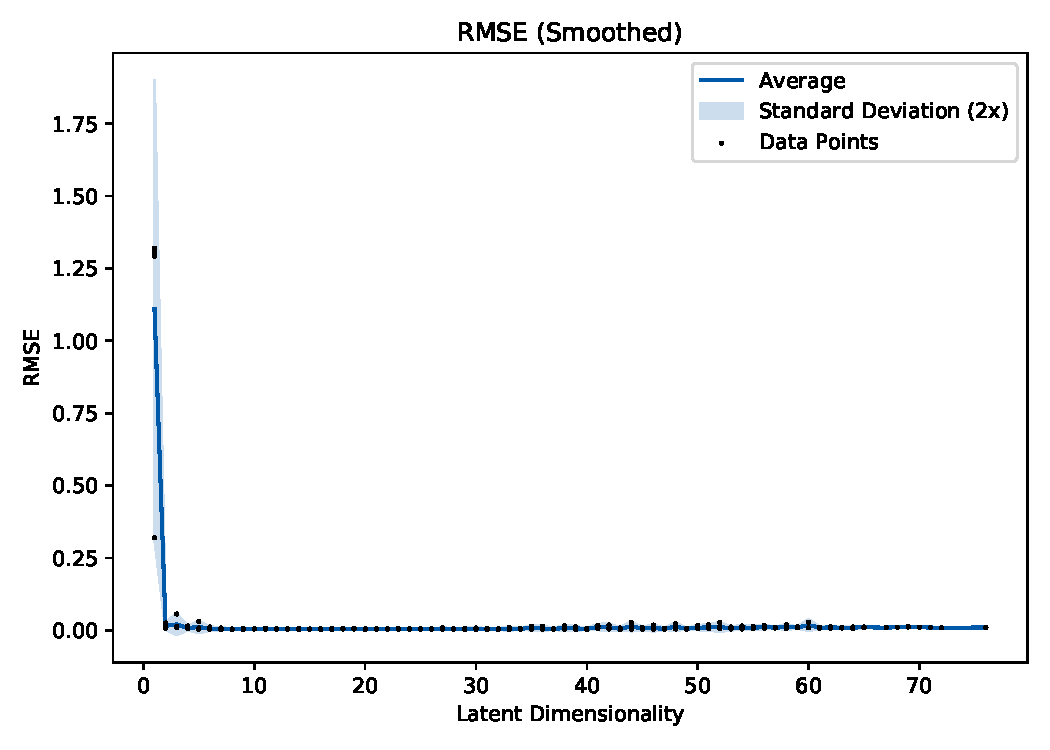
\includegraphics[width=0.7\linewidth]{figures/results/cartpole-gym/latent-dim/comparison-rmse-smoothed-mean-vs-latent-dim.pdf}
				\caption{The \ac{rmse} of the smoothed trajectory from \( t = 1 \) to \( t = T_\train \), \ac{ie} on the training data. We can see that we need at least \( 2\) latent dimensions to get decent smoothing results.}
				\label{fig:cartpoleRmseSmoothed}
			\end{figure}

			\begin{figure}
				\centering
				\begin{subfigure}{0.7\linewidth}
					\centering
					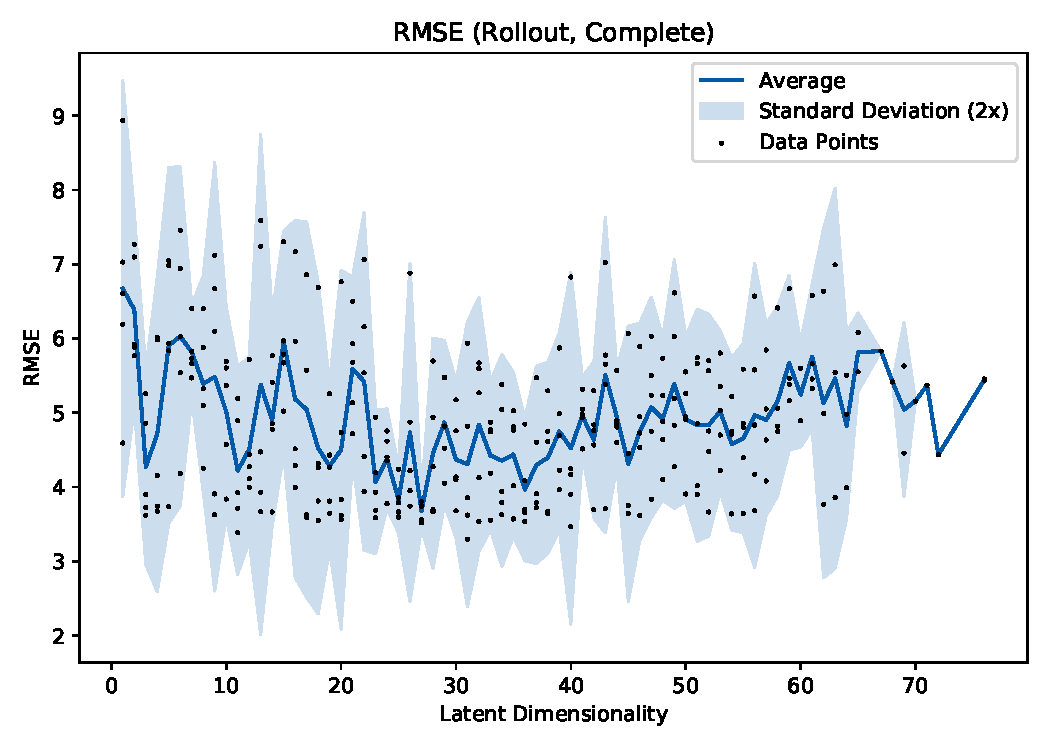
\includegraphics[width=\linewidth]{figures/results/cartpole-gym/latent-dim/comparison-rmse-rollout-mean-vs-latent-dim.pdf}
					\caption{Error of the complete rollout from \( t = 1 \) to \( t = T \) on the cartpole environment.}
					\label{fig:cartpoleRmseComplete}
				\end{subfigure} \\
				\begin{subfigure}{0.5\linewidth}
					\centering
					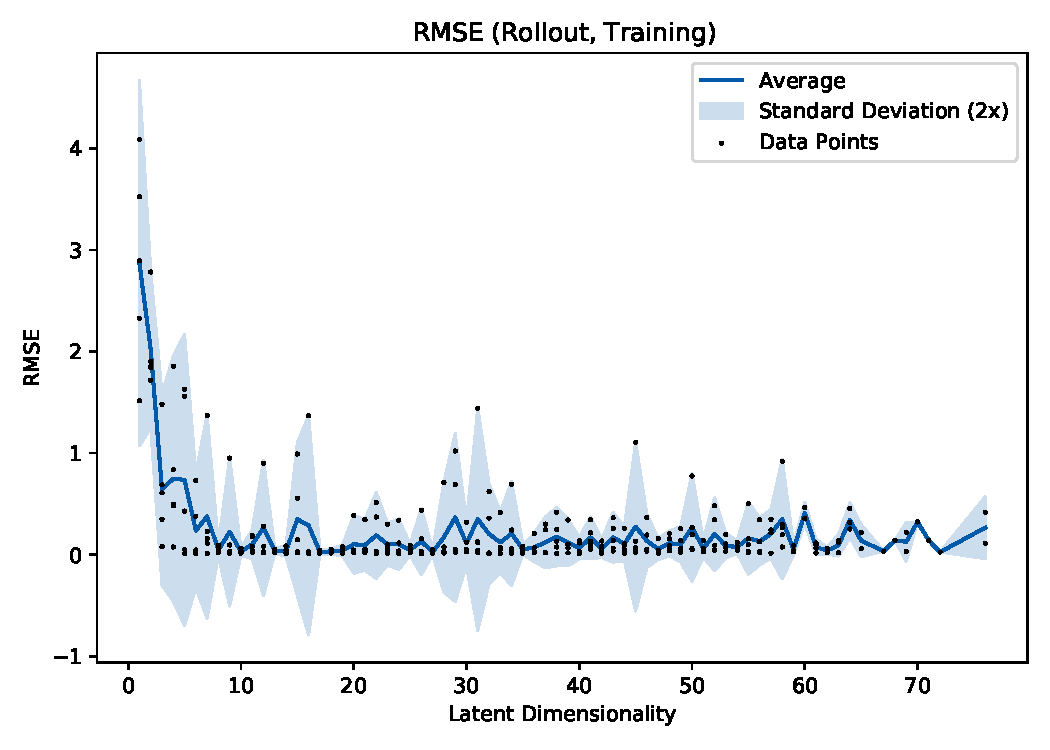
\includegraphics[width=\linewidth]{figures/results/cartpole-gym/latent-dim/comparison-rmse-rollout-train-mean-vs-latent-dim.pdf}
					\caption{Error of the rollout on the training data only on the cartpole environment.}
					\label{fig:cartpoleRmseTrain}
				\end{subfigure}%
				~
				\begin{subfigure}{0.5\linewidth}
					\centering
					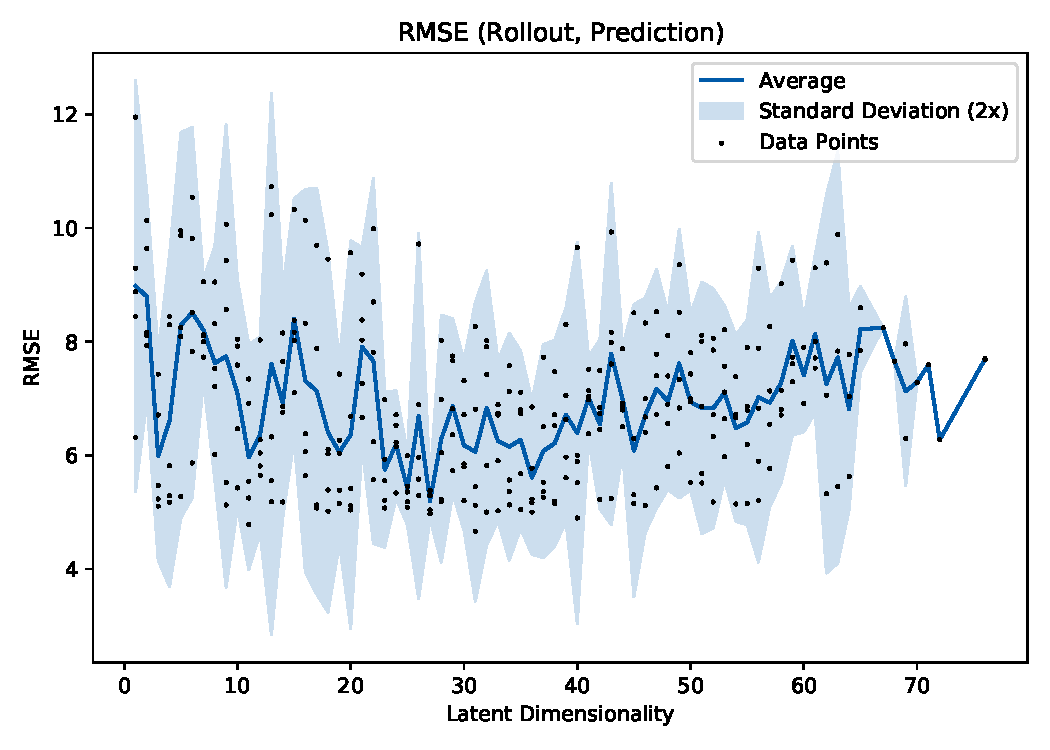
\includegraphics[width=\linewidth]{figures/results/cartpole-gym/latent-dim/comparison-rmse-rollout-prediction-mean-vs-latent-dim.pdf}
					\caption{Error of the rollout on the prediction only on the cartpole environment.}
					\label{fig:cartpoleRmsePred}
				\end{subfigure}
				\caption{Plot of the errors of the cartpole environment for different latent dimensions. The black dots show the measured data, the blue line the average of the data points at a specific time step. The blue shaded region shows two times the standard deviation. The data points on the right side of the plot get more and more sparse as the algorithm gets more and more numerically brittle for higher latent dimensionalities.}
				\label{fig:cartpoleRmse}
			\end{figure}
		% end

		\subsubsection{Exemplary Evaluation: One-Dimensional Latent}
			We will now look at an exemplary run for the latent dimensionality \( k = 1 \). As we have already seen, this should not perform well and even the smoothed trajectory should be far off.

			\begin{figure}
				\centering
				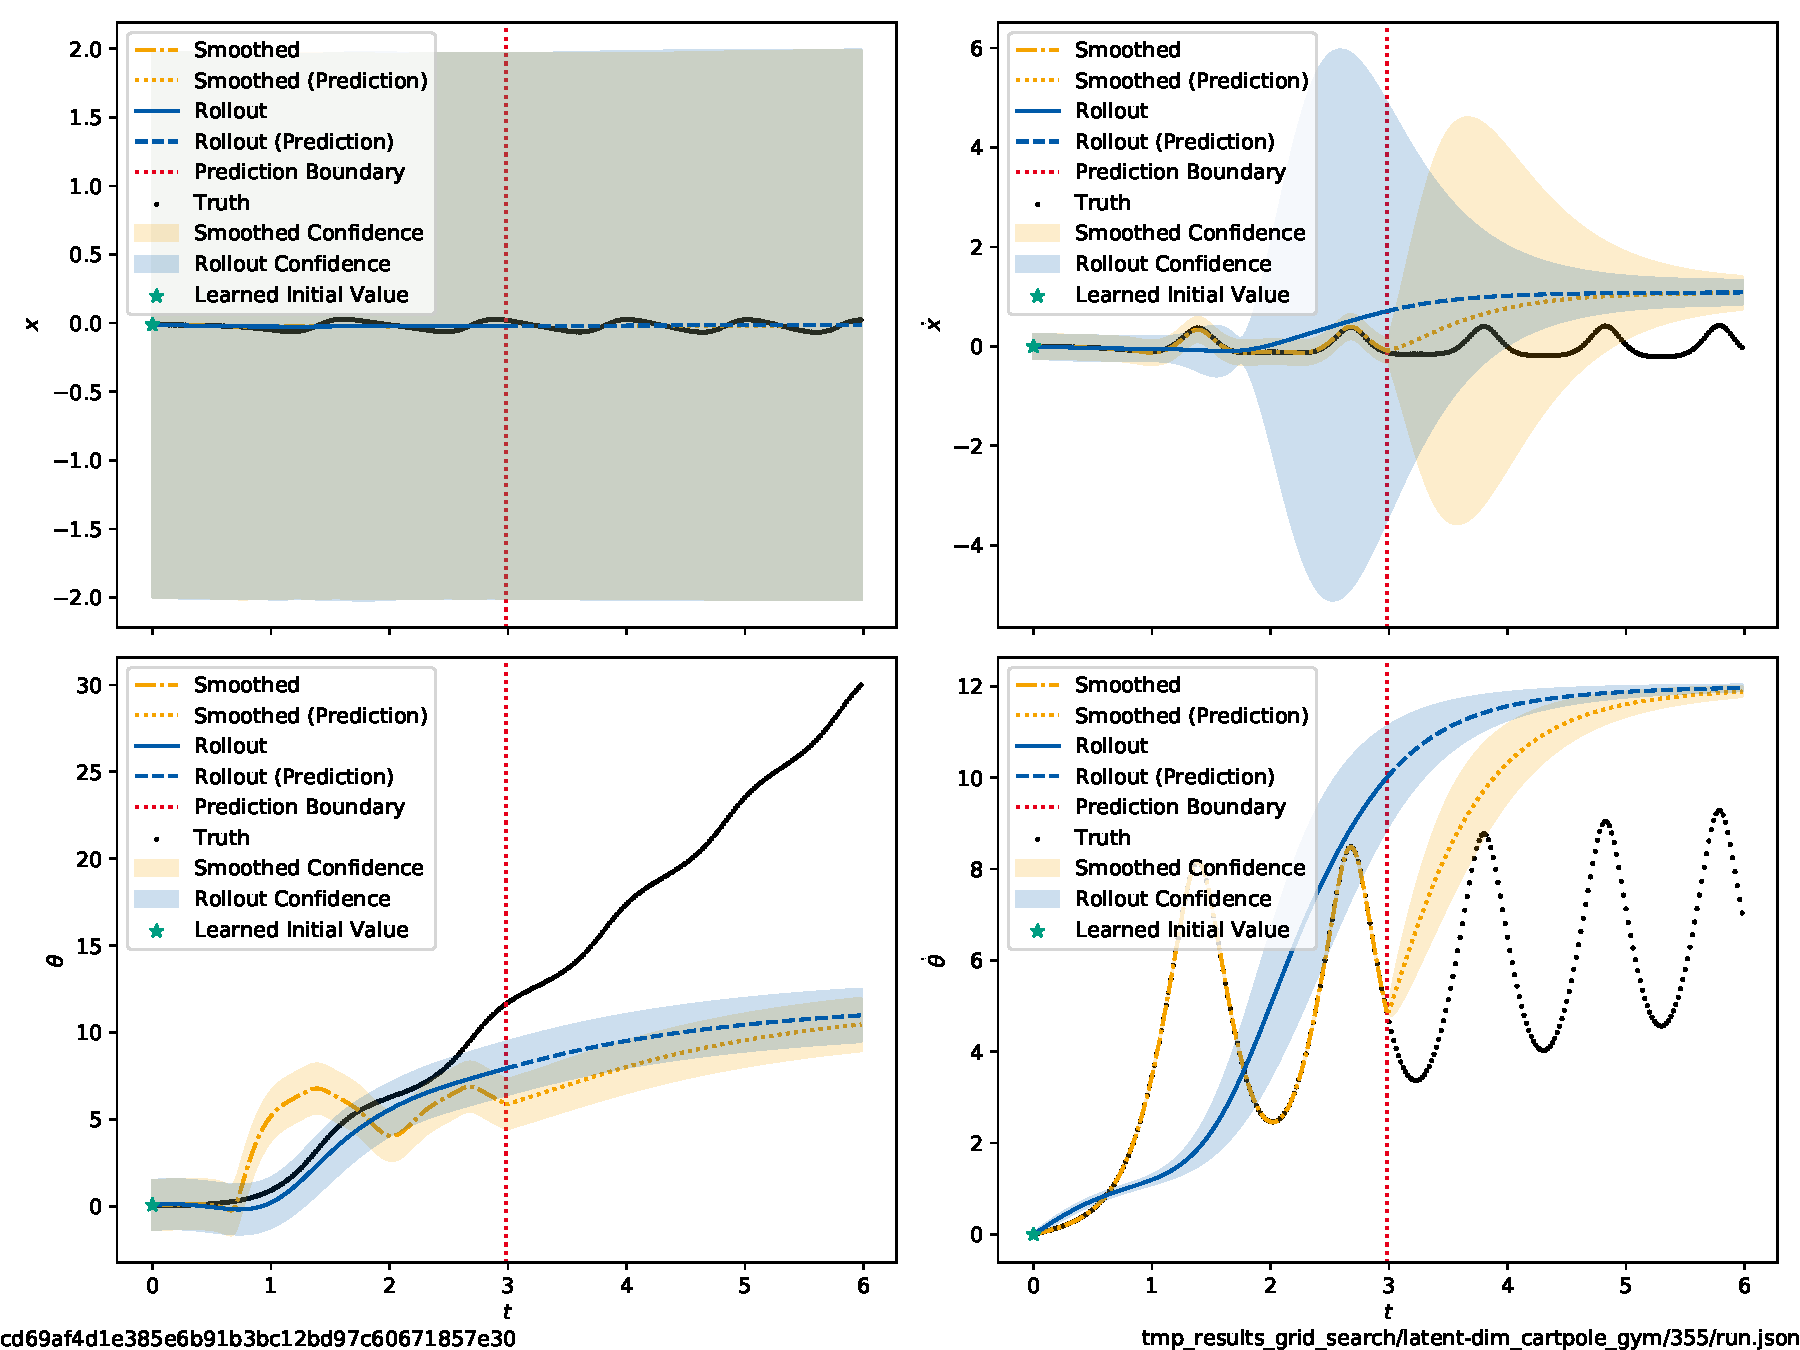
\includegraphics[width=\linewidth]{figures/results/cartpole-gym/run-latent-dim-01/rollout-observations-N0.pdf}
				\caption{TODO} % TODO
				\label{fig:cartpoleRolloutL01}
			\end{figure}
		% end
	% end

	\subsection{Gym Double Pendulum}
		\todo{Results: Gym Double Pendulum}

		\subsubsection{Influence of the Latent Dimensionality}
			\todo{Results: Gym Double Pendulum, Latent Dim.}
		% end
	% end
% end
